
%(BEGIN_QUESTION)
% Copyright 2008, Tony R. Kuphaldt, released under the Creative Commons Attribution License (v 1.0)
% This means you may do almost anything with this work of mine, so long as you give me proper credit

Sketch a circuit whereby this loop-powered pressure transmitter sends a signal to an analog voltage meter (acting as a remote pressure gauge).  Be sure to route all wiring and attach any necessary components to terminals on the terminal strip:

\vskip 50pt

$$\includegraphics[width=15.5cm]{i03181x01.eps}$$

Note: avoid connecting more than two wires to each screw terminal on the terminal strip, to avoid ``overcrowding'' any connection points, and avoid crossing wires over each other.

\vfil 

\underbar{file i03181}
\eject
%(END_QUESTION)





%(BEGIN_ANSWER)

This is a graded question -- no answers or hints given!

%(END_ANSWER)





%(BEGIN_NOTES)

As usual, a helpful strategy when sketching DC circuits is to identify components as being either {\it sources} or {\it loads} and then sketch current arrows in the appropriate directions relating to the voltage polarity for each component.  Here, you can see arrows drawn in the direction of {\it conventional flow}, pointing toward the positive terminal of each load and away from the positive terminal of the source.  After doing this, all we need to do is join arrow tips to arrow tails to form a series 4-20 mA loop circuit.  Note that the answer shown here is just one possible solution:

$$\includegraphics[width=15.5cm]{i03181x02.eps}$$

%INDEX% Pictorial circuit review (4-20 mA loop)

%(END_NOTES)


